\documentclass{standalone}
\usepackage{tikz}
\usepackage{verbatim}
\begin{document}
\pagestyle{empty}
  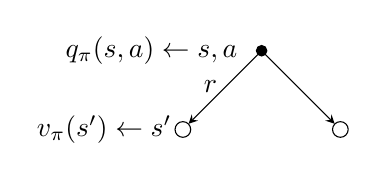
\begin{tikzpicture}
    \node[draw,circle, fill, scale=0.4] (s) at (0,0) {};
    \node at (-1.4, 0) {$q_{\pi}(s,a) \leftarrow s, a$};
    \foreach \x in {-1, 1} {
      \node[draw,circle,scale=0.6] (b\x) at (\x, -1) {};
      \draw[-stealth] (s) -- (b\x);
    }
    \node at (-2, -1) {$v_{\pi}(s')\leftarrow s'$};
    \node at (-0.65, -0.45) {$r$};
  \end{tikzpicture}

  % The graphic
  \node[draw,circle,scale=0.4] (s) at (0,0) {};
  \node at (-1.4, 0) {$q_{\pi}(s,a) \leftarrow s, a$};
  \foreach \x in {-2, 0, 2} {
      \node[draw,circle,fill,scale=0.6] (b\x) at (\x, -1) {};
      
      \draw[-stealth] (s) -- (b\x);
      \draw[-stealth] (b\x) -- (l\x);
      \draw[-stealth] (b\x) -- (r\x);
  }
  % \node at (0.2, -0.5) {$\pi$};
  \node at (-2.3, -1.) {$a$};
  \node at (-2.35, -1.45) {$r$};
  % \node[below = 2mm of b1] {$p$};
  \node at (-3.5, -2.) {$v_{\pi}(s')\leftarrow s'$};
\end{tikzpicture}
\end{document}